\documentclass{article}

\usepackage{amsmath, amsthm, amssymb, amsfonts}
\usepackage{thmtools}
\usepackage{graphicx}
\usepackage{setspace}
\usepackage{geometry}
\usepackage{float}
\usepackage[hidelinks]{hyperref}
\usepackage[utf8]{inputenc}
\usepackage[spanish]{babel}
\usepackage{framed}
\usepackage[dvipsnames]{xcolor}
\usepackage{tcolorbox}
\usepackage{tikz}
\usepackage{caption}
\usepackage{longtable}
\usepackage{xurl}
\usepackage{pdflscape}
\usepackage{listings}
\usepackage{array}
\usepackage{multirow}


\colorlet{LightGray}{White!90!Periwinkle}
\colorlet{LightOrange}{Orange!15}
\colorlet{LightGreen}{Green!15}


\newcommand{\HRule}[1]{\rule{\linewidth}{#1}}

\declaretheoremstyle[name=Theorem,]{thmsty}
\declaretheorem[style=thmsty,numberwithin=section]{theorem}
\tcolorboxenvironment{theorem}{colback=LightGray}

\declaretheoremstyle[name=Proposition,]{prosty}
\declaretheorem[style=prosty,numberlike=theorem]{proposition}
\tcolorboxenvironment{proposition}{colback=LightOrange}

\declaretheoremstyle[name=Principle,]{prcpsty}
\declaretheorem[style=prcpsty,numberlike=theorem]{principle}
\tcolorboxenvironment{principle}{colback=LightGreen}

\setstretch{1.2}
\geometry{
    textheight=9in,
    textwidth=5.5in,
    top=1in,
    headheight=12pt,
    headsep=25pt,
    footskip=30pt
}

\definecolor{dkgreen}{rgb}{0,0.6,0}
\definecolor{gray}{rgb}{0.5,0.5,0.5}
\definecolor{mauve}{rgb}{0.58,0,0.82}
\lstset{language=SQL,
  basicstyle={\small\ttfamily},
  belowskip=3mm,
  breakatwhitespace=true,
  breaklines=true,
  classoffset=0,
  columns=flexible,
  commentstyle=\color{dkgreen},
  framexleftmargin=0.25em,
  frameshape={}{yy}{}{}, %To remove to vertical lines on left, set `frameshape={}{}{}{}`
  keywordstyle=\color{blue},
  numbers=none, %If you want line numbers, set `numbers=left`
  numberstyle=\tiny\color{gray},
  showstringspaces=false,
  stringstyle=\color{mauve},
  tabsize=3,
  xleftmargin =1em
}


\newcolumntype{L}[1]{>{\raggedright\let\newline\\\arraybackslash\hspace{0pt}}m{#1}}
\newcolumntype{C}[1]{>{\centering\let\newline\\\arraybackslash\hspace{0pt}}m{#1}}
\newcolumntype{R}[1]{>{\raggedleft\let\newline\\\arraybackslash{0pt}}m{#1}}

% ------------------------------------------------------------------------------

\begin{document}

% ------------------------------------------------------------------------------
% Cover Page and ToC
% ------------------------------------------------------------------------------

\title{ \normalsize \textsc{}
		\\ [2.0cm]
		\HRule{1.5pt} \\
		\LARGE \textbf{\uppercase{Base de datos TADEO TOURS}
		\HRule{2.0pt} \\ [0.6cm] \LARGE{Requerimientos Proyecto} \vspace*{10\baselineskip}}
		}
\date{}
\author{\textbf{Alvarado Becerra Ludwig} \\ 
		  \textbf{Granados Johan Esteban} \\
		Bases de Datos - 2024-1S\\
		\today}

\maketitle
\newpage

\tableofcontents
\newpage

% ------------------------------------------------------------------------------
\section{Introducción}

\subsection{Contexto del negocio}
La agencia de viajes en cuestión se centra en proporcionar servicios de transporte aéreo, alojamiento y turismo, con un enfoque inicial en atender las necesidades de la comunidad universitaria, incluyendo estudiantes, profesores y funcionarios. Aunque su principal mercado objetivo es la población universitaria, en los últimos años ha ampliado sus servicios para abarcar segmentos como el turismo familiar y los viajes de negocios empresariales, respondiendo a las solicitudes y preferencias de sus clientes.

El proceso de reserva se realiza tanto en la oficina ubicada dentro de las instalaciones universitarias como a través de una línea telefónica de atención al cliente. Además, la agencia está considerando la posibilidad de expansión mediante la creación de un sitio web que permita a los clientes realizar reservas en línea de manera más eficiente.

El gerente expresó su interés en mejorar el proceso de reservas mediante la implementación de una base de datos unificada y la eventual automatización del proceso. Estos cambios se alinean con la visión de la agencia de viajes de mantenerse actualizada y competitiva en el mercado, brindando a sus clientes una experiencia más eficiente y conveniente.

\subsection{Antecedentes}
Debido a que estamos tratando de un proyecto de automatización en una agencia de viajes se debe analizar la competencia que ya existe para el proyecto. Uno de ellos puede ser la agencia de viajes \textit{Despegar} (\url{https://www.despegar.com.co/})

\subsubsection{Despegar}
Esta agencia de viajes líder en Latinoamérica. Se hizo con el objetivo de que los viajeros evitaran las largas colas en las ventanillas de los aeropuertos para poder conseguir un vuelo. 

La agencia permite realizar alojamientos, vuelos, paquetes, ofertas, alquileres, actividades, circuitos, carros, traslados, servicio de asistencia y muchos más servicios. Para el caso de \textit{TADEO TOURS} comparte que brinda servicios de transporte aéreo, alojamiento y turismo, pero centrado en la comunidad universitaria. Mientras que \textit{Despegar} se centra en el viajero. Ahí se podría remarcar la diferencia entre ambas agencias, esto permitirá a \textit{TADEO TOURS} centrar sus planes en universitarios, académicos y funcionarios. Dando una experiencia más personalizada para este grupo de personas, por ejemplo, para universitarios podría incluir paquetes especializados para \textit{parches} entre amigos, para académicos puede incluir viajes para conferencias de investigación y así sucesivamente.

\subsection{Justificación}
Este proyecto implementará una base de datos que sea eficiente tanto para la universidad como para el usuario. Utilizando una base de datos relacional se permite almacenar la información de manera organizada y así automatizar el proceso de reserva y todas las tareas que lleva consigo \textit{TADEO TOURS}. Al utilizar estos procesos de automatización, se ahorra la intervención humana, esto no es algo malo para los trabajadores. Es beneficioso tanto para la agencia como para estos trabajadores, al permitir estos procesos de digitalización se evita el error humano en la introducción de datos (algo que es frecuente cuando se hacen estas reservas por un humano) y también lleva al trabajador a que se forme en saber utilizar estas tecnologías. Este proyecto se alinea con la visión a futuro que posee la agencia de proporcionar servicios de alta calidad y adaptarse a las demandas del sector de viajes. 

\subsection{Generalidades}
A grandes rasgos, el proyecto debe estar en la capacidad de poder abordar las siguientes acciones y actividades:
\begin{itemize}
    \item Almacenamiento de detalles de cada reserva, incluyendo destinos, fechas de viaje, preferencias del cliente y tipo de alojamiento.
    \item Seguimiento del estado de las reservas (pendiente, confirmada, cancelada) y fechas límite de pago.
    \item Creación de perfiles individuales para cada cliente, que incluyan información personal, preferencias de viaje, historial de reservas y datos de contacto.
    \item Programación de recordatorios automáticos para clientes sobre fechas límite de pago y detalles de viaje.
    \item Registro de todas las actividades realizadas en la base de datos, proporcionando una pista de auditoría para rastrear cambios y asegurar la responsabilidad.
\end{itemize}


\section{Objetivos}
Los objetivos se dividen en:
\begin{itemize}
    \item \textbf{Proyecto:} 
    \begin{itemize}
        \item Crear un sistema centralizado que almacene y gestione eficientemente la información de reservas, clientes y proveedores
        \item Implementar un sistema que permita automatizar tareas rutinarias asociadas con la gestión de reservas, como consultas de disponibilidad, confirmaciones y recordatorios de pago.
    \end{itemize}
    \item \textbf{Negocio:}
    \begin{itemize}
        \item Reducir el tiempo dedicado a la gestión manual de reservas mediante la automatización de procesos, lo que permitirá una mayor eficiencia operativa.
        \item Mejorar la relación con aerolíneas y hoteles mediante una gestión más eficiente de reservas y pagos, posiblemente facilitando negociaciones y acuerdos futuros.
    \end{itemize}
    \item \textbf{Académico:}
    \begin{itemize}
        \item Utilizar los conocimientos adquiridos en bases de datos para planificar, ejecutar y controlar la implementación de la base de datos y la automatización del proceso.
        \item Investigar y evaluar tecnologías apropiadas para el desarrollo de la base de datos y la automatización del proceso, adquiriendo experiencia práctica en la toma de decisiones tecnológicas.
    \end{itemize}
\end{itemize}

\newpage
\section{Alcance del proyecto}
Diseñar e implementar una base de datos centralizada que almacene información sobre clientes, reservas, proveedores (aerolíneas y hoteles), y cualquier otro dato relevante para el proceso de reservas. Implementar un sistema que automatice tareas asociadas con la gestión de reservas, incluyendo consultas de disponibilidad, confirmaciones, recordatorios de pago y la generación de documentación asociada. Reducir la dependencia de procesos manuales y minimizar los tiempos de respuesta, mejorando así la eficiencia operativa en la gestión de reservas.

Sin embargo, este proyecto no cubre; el desarrollo de un sitio web de reservas en línea, La implementación de un sistema de pagos en línea, cambios significativos en los procesos que lleva la agencia actualmente.

\newpage

\section{Modelo de Datos}
Los nombres de las tablas se van a colocar en fuente \textit{\textbf{CURSIVA NEGRILLA}} y los atributos de la tabla serán colocados únicamente en letra \textit{CURSIVA}. Esto debido a que se facilita mucho más en la lectura de las tablas, después se representará gráficamente mediante diagramas de relación y entidad-relación.
\subsection{Normalización en 1FN}
Por el momento, lo que se tiene de base de datos es una tabla con muchos atributos. De acuerdo a los requerimientos del cliente se obtiene la tabla \textit{\textbf{Reserva}}, la tabla a priori va a tener los siguientes atributos:
\begin{itemize}
    \item \textit{\textbf{Reserva}(Alojamiento\_Preferencia, Hotel\_Reservado, Estrellas\_Hotel, Fecha\_Ingreso\_Hotel, Fecha\_Salida\_Hotel, Precio\_Reserva\_Hotel, Sitio\_Preferencia, Fecha\_Limite\_Pago\_Reserva, Opcion\_Pago\_Hotel, Estado\_Solicitud\_Hotel, Tipo\_Acomodacion\_Hotel, Aerolinea\_Preferencia, Aerolinea\_Reservada, Fecha\_Salida\_Vuelo, Fecha\_Regreso\_Vuelo, Hora\_Salida\_Vuelo, Hora\_Regreso\_Vuelo, Tipo\_Vuelo, Fecha\_Limite\_Pago\_Tiquete, Opcion\_Pago, Estado\_Solicitud\_Vuelo, Ciudad\_Origen, Destino\_Viaje, Fecha\_Registro\_Reserva, Nombre\_Completo\_Acompañante, Documento\_Cliente, Edad\_Cliente, Correo\_Cliente, Telefono\_Fijo\_Cliente, Telefono\_Celular\_Cliente, Direccion\_Cliente, Ciudad\_Residencia\_Cliente, Numero\_Fax, Nombre\_Completo\_Acompañante, Documento\_Acompañante, Edad\_Acompañante )}
\end{itemize}

Para que una tabla se encuentra en 1FN esta no debe contener atributos multivariados, compuestos o sus combinaciones. El atributo \textit{Nombre\_Completo} tanto del cliente como del acompañante está compuesto por el nombre inicial y los apellidos, por lo tanto, toca dividir este atributo en nombres y apellidos. También ocurre con los documentos de los usuarios, no sé sabe si se trata de una tarjeta de identidad, cédula, pasaporte u otros. También, para este tipo de normalización, se pide que se eliminen los grupos repetidos y que se cree una nueva tabla con PK de la tabla base y el grupo repetido. Los grupos que se ven repetidos son: La reserva del hotel, la reserva del vuelo, reserva del servicio y el cliente. Por lo tanto se crean las tablas que se muestran en la figura \ref{fig:NormalizacionFN1}.
\begin{itemize}
    \item \textit{\textbf{Reserva\_Hotel}(ID\_Hotel\_Reserva, Alojamiento\_Preferencia, Hotel\_Reservado, Estrellas\_Hotel, Fecha\_Ingreso, Fecha\_Salida, Precio\_Reserva, Sitio\_Preferencia, Fecha\_Limite\_Pago\_Reserva, Opcion\_Pago, Estado\_Solicitud\_Hotel, Tipo\_Acomodacion)}
    \item \textit{\textbf{Vuelo\_Reserva}(ID\_Vuelo\_Reserva, Aerolinea\_Preferencia, Aerolinea\_Reservada, Fecha\_Salida, Fecha\_Regreso, Hora\_Salida, Hora\_Regreso, Tipo\_Vuelo, Fecha\_Limite\_Pago\_Tiquete, Opcion\_Pago, Estado\_Solicitud\_Vuelo)}
    \item \textit{\textbf{Reserva}(ID\_Reserva, ID\_Cliente, Ciudad\_Origen, Destino\_Viaje, ID\_Vuelo\_Reserva, Fecha\_Registro, ID\_Hotel\_Reserva)}
    \item \textit{\textbf{Cliente} (ID\_Cliente, Nombre(s), Apellido(s), Tipo\_Documento, Documento, Edad, Correo, Telefono\_Fijo, Telefono\_Celular, Direccion, Ciudad\_Residencia, Numero\_Fax, Nombre(s)\_Acompañante, Apellido(s)\_Acompañante, Tipo\_Documento\_Acompañante, Documento\_Acompañante, Edad\_Acompañante )}
\end{itemize}



Una normalización en FN1 no debe presentar atributos multivariados, compuestos o sus combinaciones. En este caso, la tabla tiene atributos como \textit{Nombre\_Completo} que está compuesto del nombre y apellido, entonces se crean dos atributos para quitar el que se tiene, los cuales son \textit{Nombre(s)} y \textit{Apellido(s)}, esto para quitar esa composición. Por otra parte, el atributo \textit{Documento\_Identidad} está conformado por pasaporte, cédula, tarjeta de identidad, y se necesita saber qué tipo de documento de identidad posee el usuario, por lo tanto, se agrega otro atributo de \textit{Tipo\_documento}. Esto se repite con los acompañantes del usuario que está haciendo la reserva, añadiendo campos como: \textit{Nombre(s)\_Acompañante, Apellido(s)\_Acompañante, Tipo\_Documento\_Acompañante} y \textit{Documento\_Identidad\_Acompañante}. 

Por otra parte, toca eliminar los grupos repetidos y crear una nueva tabla con la \textit{primary key} de la tabla base y el grupo repetido. Por lo tanto, las tablas que quedan son las que se muestran en la figura \ref{fig:NormalizacionFN1} de la sección anexos.
\begin{itemize}
    \item \textit{\textbf{Hotel}}(\textit{ID\_Hotel, Nombre\_Hotel, Estrellas\_Hotel })
    \item \textbf{\textit{Aerolinea}}(\textit{ID\_Aerolínea, Nombre\_Aerolínea, Tipo\_Vuelo})
    \item \textbf{\textit{Reserva}}(\textit{ID\_Reserva, ID\_Cliente, Ciudad\_Origen, Destino\_Viaje, Fecha\_Salida, Fecha\_Regreso, Hora\_Salida, Hora\_Regreso, Tipo\_Vuelo, Aerolínea\_Preferencia, Alojamiento\_Preferencia, Sitio\_Preferencia, Fecha\_Limite\_Pago\_Tiquete, Fecha\_Limite\_Pago\_Reserva, Precio\_Tiquete, Precio\_Reserva, Opcion\_Pago, Fecha\_Registro, Estado\_Solicitud\_Reserva, Estado\_Solicitud\_Vuelo, Aerolinea\_Reservada, Hotel\_Reservado})
    \item \textbf{\textit{Cliente}}(\textit{ID\_Cliente, Nombre(s), Appelido(s), Tipo\_Documento, Documento, Edad, Correo, Telefono\_Fijo, Telefono\_Celular, Direccion, Ciudad\_Residencia, Numero\_Fax, Nombre(s)\_Acompañante, Apellido(s)\_Acompañante, Tipo\_Documento\_Acompañante, Documento\_Acompañante, Edad\_Acompañante)})
\end{itemize}





\subsection{Normalización en 2FN}

\begin{enumerate}
    \item Para la normalización 2FN se requiere determinar cuáles columnas que no son llave no dependen de la llave primaria de la tabla. 
    \item Eliminar esas columnas de la tabla base.
    \item Crear una segunda tabla con esas columnas y la(s) columna(s) de la PK de la cual dependen.
\end{enumerate}

Las tablas \textit{\textbf{Reserva\_Hotel}} y  \textbf{\textit{Vuelo\_Reserva}} poseen atributos como la información de los hoteles, estas columnas no dependen del ID de las reservas, por lo tanto, se crean las tablas \textit{\textbf{Hotel}} y \textbf{\textit{Aerolinea}}. Los acompañantes del cliente van a ir listados en una tabla aparte, en donde se asocie el \textit{ID\_Cliente} para que se identifiquen con el cliente al cual van asociados, así entonces, se crea la tabla \textit{\textbf{Acompañante}}. Por lo tanto, el modelo queda listado tal como muestra la figura \ref{fig:Normalizacion2FN} de la sección anexos.
\begin{itemize}
    \item \textit{\textbf{Hotel}(ID\_Hotel, Nombre\_Hotel, Estrellas\_Hotel, Reservas)}
    \item \textit{\textbf{Aerolinea}(ID\_Aerolinea, Nombre\_Aerolinea, Reservas)}
    \item \textit{\textbf{Reserva\_Hotel}(ID\_Hotel\_Reserva, FK-Alojamiento\_Preferencia, FK-Hotel\_Reservado, Fecha\_Ingreso, Fecha\_Salida, Precio\_Reserva, Sitio\_Preferencia, Fecha\_Limite\_Pago\_Reserva, Opcion\_Pago, Estado\_Solicitud\_Hotel, Tipo\_Acomodacion)}
    \item \textit{\textbf{Vuelo\_Reserva}(ID\_Vuelo\_Reserva, FK-Aerolinea\_Preferencia, FK-Aerolinea\_Reservada, Fecha\_Salida, Fecha\_Regreso, Hora\_Salida, Hora\_Regreso, Tipo\_Vuelo, Fecha\_Limite\_Pago\_Tiquete, Opcion\_Pago, Estado\_Solicitud\_Vuelo)}
    \item \textit{\textbf{Reserva}(ID\_Reserva, FK-Id\_Cliente, Ciudad\_Origen, Destino\_Viaje, FK-ID\_Vuelo\_Reserva, Fecha\_Registro, FK-ID\_Hotel\_Reserva)}
    \item \textit{\textbf{Cliente}(ID\_Cliente, Nombre(s), Apellido(s), Tipo\_Documento, Documento, Edad, Correo, Telefono\_Fijo, Telefono\_Celular, Direccion, Ciudad\_Residencia, Numero\_Fax )}
    \item \textit{\textbf{Acompañante}(ID\_Acompañante, FK-ID\_Cliente, Nombre(s), Apellido(s), Tipo\_Documento, Documento, Edad )}
\end{itemize}


\subsection{Normalización en 3FN}

Para esta normalización se requiere de:
\begin{enumerate}
    \item Determinar las columnas que son dependientes de otra columna no llave.
    \item Eliminar esas columnas de la tabla base.
    \item Crear una segunda tabla con esas columnas y con la columna no llave de la cual son dependientes.
\end{enumerate}

Finalmente, se crean diferentes tablas para las habitaciones de los hoteles, bancos, métodos de pago, solicitud crédito, ciudades y países. Esto con el fin de eliminar por completo la redundancia de la tabla. Por lo tanto, las tablas listadas en el modelo normalizado en la tercera forma normal es el que se presenta en la figura \ref{fig:Normalizacion3FN} de la sección anexos, las tablas y atributos se listan a continuación. 
\begin{itemize}
    \item \textit{\textbf{Habitaciones}(ID\_Habitacion, Numero\_Personas, Tipo\_Habitacion)}
    \item \textit{\textbf{Banco}(ID\_Banco, Nombre\_Banco, Telefono)}
    \item \textit{\textbf{Hotel}(ID\_Hotel, FK-ID\_Ciudad, Nombre\_Hotel, Estrellas\_Hotel, Reservas )}
    \item \textit{\textbf{Aerolinea}(ID\_Aerolinea, Nombre\_Aerolinea, Reservas)}
    \item \textit{\textbf{Metodo\_Pago}(ID\_Metodo, Metodo\_Nombre, FK-ID\_Banco)}
    \item \textit{\textbf{Solicitud\_Credito}(ID\_Solicitud\_Credito, FK-ID\_Banco, FK-ID\_Cliente, Estado\_Solicitud, Fecha\_Registro, Cantidad)}
    \item \textit{\textbf{Reserva\_Hotel}(ID\_Hotel\_Reserva, FK-Alojamiento\_Preferencia, FK-Hotel\_Reservado, Fecha\_Ingreso, Fecha\_Salida, Precio\_Reserva, FK-Sitio\_Preferencia, Fecha\_Limite\_Pago\_Reserva, FK-Opcion\_Pago, Estado\_Solicitud\_Hotel, FK-Tipo\_Acomodacion )}
    \item \textit{\textbf{Vuelo\_Reserva} (ID\_Vuelo\_Reserva, FK-Aerolinea\_Preferencia, FK-Aerolinea\_Reservada, Fecha\_Salida, Fecha\_Regreso, Hora\_Salida, Hora\_Regreso, Tipo\_Vuelo, Fecha\_Limite\_Pago\_Tiquete, FK-Opcion\_Pago, Estado\_Solicitud\_Vuelo)}
    \item \textit{\textbf{Reserva}(ID\_Reserva, FK-ID\_Cliente, FK-Ciudad\_Origen, FK-Destino\_Viaje, FK-ID\_Vuelo\_Reserva, Fecha\_Registro, FK-ID\_Hotel\_Reserva, Valor\_Total, Estado\_Reserva )}
    \item \textit{\textbf{Cliente}(ID\_Cliente, Nombre(s), Apellido(s), Tipo\_Documento, Documento, Edad, Correo, Telefono\_Fijo, Telefono\_Celular, Direccion, FK-Ciudad\_Residencia, Numero\_Fax, FK-ID\_Solicitud\_Credito )}
    \item \textit{\textbf{Acompañante}(ID\_Acompañante, FK-ID\_Cliente, Nombre(s), Apellido(s), Tipo\_Documento, Documento, Edad )}
    \item \textit{\textbf{Ciudad}(ID\_Ciudad, ID\_Pais, Nombre ) }
    \item \textit{\textbf{Pais}(ID\_Pais, Nombre )}
\end{itemize}

Por último, se han establecido las relaciones entre las tablas, se pueden ver en la figura \ref{fig:EntidadRelacion}, sin embargo, si se desea observar en más detalle el modelo, puede dar clic \href{https://viewer.diagrams.net/?tags=%7B%7D&highlight=0000ff&edit=_blank&layers=1&nav=1&title=Diagrama%20sin%20t%C3%ADtulo.drawio#R7Z3Zctu4EoafRlVzLpwiSJGULmNbmWQmWyVTmeRKRYu0jYQSNBTlJU9%2FSImLJEAUYXHB0qem6lgMScvAj%2F7QjUZjYF3Nn%2F6MvOX9B%2BIH4cA0%2FKeBdT0wTQs54%2BT%2F0ivP2yvIQmh75S7C%2FvaaUV74in8H2Y351TX2g1V2bXspJiSM8XL%2F4owsFsEs3rvmRRF53L%2FtloT%2B3oWldxfsfY30wteZFwbUbf9iP77fXh3ZO3e%2FDfDdff6bkZH9y9zLb84urO49nzzuXQqe4jdkEWdf8XMQzb1FsIiTf%2FngRb%2BCaGBP7uM4%2FUtfD8w3yX%2B36d2v7gi5CwNviVevZmSeXJ6tklve3HpzHKbtvPOiy%2BxFya%2BzJgPrKiIk3v40f7oKwrSz9rvhzZF%2FLdohSt9b44Gri4fn97%2BMePH20foWf%2Fhw99m9uTCt7WsevHCdNfCXYBVED17WRvFz3vBJcy3TH2PvJr10uYq9KM70YRnJhaTHYw8vkj%2FOukabz2HoLVd4c%2Fv2yj0O%2FffeM1nH%2BYvyT5e3%2BCnwv2zlkd6bKOV98rL0Y%2FrytKG%2FZl8m%2FWcvxHeL5OdZ8tenv%2FEyClbJd3nvreLsDrp9siZ7CKI4eNq5lLXXnwGZB3H0nNyS%2F%2BsoeyQfLE72%2BbFUnpkr735HdRYyX1m269ojxzSc0djJ9J8J6674TWV%2FJT9kXcbTfUOq%2B472W9ISMfbCL8mg9BZ3my7c76G0mf2ILP%2Fxorsgzi4sCU4bePIQbIfFpi9wGF6RkKQdvSCLIL9t89fZl8l%2FSZNcGa%2FsgZ18gavkMyo%2FJ%2F%2Blt0fxFVms4igRTPqrgqTfHoO07y5jssx%2BTxjc5l8jyto2%2FfmGxHEyyo71crXOT%2Fd91teWUbOrjbb61qb69vPfPL1Lkj%2F2NtxYuHvs%2B8FiO0ZTq%2ByVPc7oTGYPFK1%2B2B2HI7Nujwxr98hOF1icPZC9rGwW7rd5YSL%2FhRcHl2S98FdUtxbf84yedqiefnc9PWWH%2B%2Bvx3PZu771cLb0ZXty93z7pdCKJp8HRQWo2KpFar2tWI%2B%2FM4cXH7zfWu4vPj5Ydv39%2FY6ELe1Tf0m86%2B0sqg8t7EuHfKZfDrO92qb35%2FIjnYTI3eRt4%2FsGlS7KZJB6RTF12dA0Fo00oOB1CgS2DMSWDN1xQaBkAxhEr9HiP4%2BBrYijSmx4T1yTVZjwPjxqI6kGgFTOYTZErcUcI2J%2FOQpzOh3sWBBcfhFGMykj5a331n%2FWvFTz8Dr9%2F%2FPTjEX%2Fy%2F7pwgSj9E2XcIVGYKqDnFb0DJfBx%2Fj50xDrQ%2FVEpca14wWwJet5whde%2B508%2FJS2fNKngxOhEA9oRANGTCEBA5whAZl0GoOOCO4sB%2BRKAmhAoVH4%2BBSo64AUUOHhbFwPepDr6OhkLeEGm37D3U3jHoRsV8HLgxaqo9boOZGHToWbgQPccsGuvLrXEAZsORCvEgULlwAGb9v2xP31YByGZRvzrDpKhgEMI2qHApR1FQEH3KBiZNVHQWliIwzWUDQSFxiEsNGJ4fsHs3pt%2BCe5wMkKIwhjgkIF2kaExR2IRYKAtDJiobwyMac9QIY9grGUOErspGDlI%2FvSexEGogUfAIQSVURDZEzKZ458%2FVu4Qvwv%2Fnvz%2BdX3hQHBIBBQMO0QBWwe0hZARBNUa1woE7KagQ0PfvKSTpjFJx7ISDDhXA%2FoxALJPRWCA2zsDOKKD0jFAy%2BRSZlO4dPBvkgxdX7HFgXNloDIGmNm0iMbA1YmMY1l2C1amFnNvHLRR5lAWS7s2rRFk0Z06NBsw3ey%2Bg4WdegjnyC5H9W1Fxa5Clg5a20Bi0qadb1dhBzsI29sOgLRc%2BWELgV75kXMDiS2KYo5PB9CIc4hXK6jW67qQkAlIOcMrbAgprD2J3SKFriHRs%2F2o4RQ2Yx2KEQA8YZSi%2BEjmN1Hwx%2Bp%2FouNECIHohw9YWBIAH6wNiN3iQ8Z1pYasg5bLTuymoJedXi%2BT57BP9AZIE6tSqgIEVqUEAAhz%2B2K3BJFxVaoh86DlohWzKfJfuaOCf%2FCSTH0yW8%2BTVpQylblzlWgHEYuOgwJEuoeI3TdELI5gpjAQqdkfVv0FTOUpQQcrr2UGRPMK0I8AsNdFBAKMeicARzxSOgJoudOF3RR0vHHiJyNUYePfxO4WVY0%2FVEEUwPgXp0v0Z%2Fw5YonSGX8tyyCym4JRB5FEUaD03L%2BJCoiKmv8hR5kLMP%2Btmf9h3%2BZ%2FyBEFlM38FxoH859vot1dIwiS3iALMr3FP1WmAIcK9KMARwYjUKA1Cri9U%2BDc47REpkD97abKU4AO9BUUmAXhOvQilUFQXwj6gYAjFxFA0BYILKN3EHBEBaUDgVO7P5QHAR30u8ZRMJvhwZU1uLQUORbjXBnohwHYKy0CBnrfLJ0nJUlf%2FbBa5QACmw7%2FZccjpYUikladYUVqnpyrBO1YYNMhQ2BB9yzofZezLeMu55r9UWgcSGAztjGv50FEprfek8II4JCAyghglgSD%2FFARCNDlRmWmDFQphV6pca0IwC4ASHUz9qcrEuIZjtf%2BdBalja7ISvGZUlCZBGyzZdBG4Mu2JOa2Vn41GA4goH4dxAuUVw2vLIToMjrXMV7lRRSbr4VowDpPPaTzVEoz6pcqqKqGyBJDW04dMuiFHp3KIRqwFlS2Bb0YJNsJKB2WReRQTtUsgXOwn5ol1HhdJ1KC9aPmPUZ%2BvDBjhp3ipTh0Wi6fsSkbAQtMpRLoFabXIfnpzdN6u2S6jILbIJJ2nal7wegHlfwsQIBKr1BhhiG7hQq9EqURVIphAFBBiF6ZeLvrr%2FhShim7F4qGMIHSiSLAhF07sVuayFg8sbYNgPKIRVswTn7ZHvWeWOSEF1KiogUd6McCxkkwwIIeWMAsgdgpC%2FKOV5IFHKuX6rOA4UJuWLBKzLAvZQiqBRloiAJIdRMCBcxaiN2iQOFiiKXMAQWIcfzK5yiYYcXO%2Bj1bCPrBgFFQH2DQPQzYtRE7hQGjRr4MKw51%2B6QQOuAAMcrgf8Uxln6FugUt6EcEG1YNhCACs1xip0SwVV41sGHVoGgLh54EbiNFIZ7jOJguvTstPAUOTejHBQeKqAvBBWYBxU654NAzBJU8BQcqqZdtQU8BPi1nmCw2TFCZBRwq0I8FLtTSFYEF7BqKnbLAVbiabilzIAFy6bWiSTJ8fbKzbb56d7QCUOAQhIZQgA1xQkCh%2Fw3XI0Y8QSEHoRA6YAGN6FWjzYHc3ozMie%2BlroLSQIDNbMcbh3EM77d1EJ4OJTLrqJgD9euoZGrKLLk9GjIsuc3oXMdsy5TDubk1oc6za8mqP43MoW7WVEJ76QH0%2FF%2BnIipwtu5OWzCrpz3UMu2CML%2FDIioNHczLOdhPTRFqvK4TKcGiUvM%2BIz9enP7xIueaUlM2Apacyragw0ivg4iEyUzdkz1BrXu56IcUOO1XCKSMe0cK47hfjZACBwLvtIVZgZS8jIrOQGno3GBFgQLJDiIApdi43iNRZEx2aMpEQC5E2RaMUyIk31nfvUo0BAkUpBcCJHb%2FIFH46GEEZw%2FvtAUjrLkhRRTcqV6Pq6HDhxVlASTLCcGCUe8sYJw%2FrBALIFWu7Gg6HvmWRDI7DS2oQD8SwNnDQpDARP2TQOHThxEcP7zTFqyS7pEWTkFDRxArigKOenyAgvZQMOwfBRyhQvlQUH9Pk%2FoooCOBm%2F0zm2xapUFQXwT6gcCBau1CgMDtHQR5Zq6SIChkDiBAzrFq7bs1uGL83zqIA5W5wKEJ%2FbiQ134CLvTKBcvonQuunMmtdfukEDqQAeWTEP1qcHGoQEMWQDaRECzof2u2q3I2kQvZRGVb0NlEVA0u5QNHHILQDwp5OsvhYcHVZDiggGUMVC%2B1YucB9rzUisuQCGPUF5a9haJZsM2kHs958tGL8cDh29VTQovV0%2BjVYZ0qrYxgo0nZFvSCMJakzGaHFVY4FFMxI7AbVVCt1zUrociekMkc%2F%2Fyxcof4Xfj35Pev6wtIKahJFR4vkZ8qTodUYeuAjhb0Hi%2FcNRFGUyaiehRoxRR2U9DBggQpM7z2k4EsEVOEEYzKSDli%2FiDyKAJTxnWZ0p7LKmPgsalJZ3NxyYr%2BeQFSDt7WiUGg45IfyfwmCuRwVcRQCS9HXqyaWq%2FrRDawB1IEjhTHwPcX8spRpiVIYItkqQM6q2WSjJ3kUW8FLGlkF6WaPonJKMkDLOmBJXbfLDF5quwIw5KaPVLKHGBhMorofNnWclzJSIkWJKAyBphhuzFEpoSgwKhDCrCFQNuG3pc7XoSBaplrRQF2U9Chp684xopkwJ3b%2ByoD4IgHSfsBRannahQMtE%2BCswxUz2wjs71IEBC8%2BSy4cf0pozBZcAyC65QFpyfij7QFzXjsT72TZl0Q1HeYCQdTg6rGgeWm5p1DfrR0mQrHjqAYGq82jWG1qdQBvdqUpS1IwxYxlKIdS0xGXW9gSfcsqZ0C195qE8ekQhiW1OyQUuUAC5NRpluL1ab6EtCPAgZNAW9G5ktvcGUNLpG3qCjVpGfMcWRkNj6vsDaqacHNYXvuAPiFjYccy6EhT8jRRLSJ1yjkWI4DoL2JaNcwDTnWNe6CgL%2B7yCOPePSbJzCONAfCnOktvoAw%2FUceGWeT956W0sqmyhPjAAhjMk4nT%2FfhhjiQDCziaEY%2FsORn1gBYegVL%2F2FIJOPRQQ1ZiGIQAFVMRNeO2i5p%2FbH6n%2BhQEUMiGkIEtk6JAJEiqbJHisi4daopEwE7q8q2oHMvXy%2BTB7FPNOcI7L2qaBzIiRCCI3b%2FHJExKaIpEwE5E0Vb5DOaw8PtfDJbz5N2lHKXVvc60Q8lFuwCEgIldbMz2kOJJWOJubo9YsEmn7It6NnjtcyYaEED%2BnEgP4gZONArB4rMqB5XzmVc4KjbI4XMgQPmkF7BmEhQmrqj7tcPATadJ%2FEhiIlPqk8%2F1DO9%2BsK2s9BLfq5RfqxwfyUdTBsgXg%2FiPOEDu742hMmvtmmG65Rfbdc388pT3qYpj%2F3pfGPYRUd9h1nVHJLRcGYAeQvNO4f8XOk%2Fq5pxtlHPNqS75SY9TzY60hZ0rHhLlOlikwMnOljEkIl%2BIHHoyQiApHuQ9J9F7dAzit635zQYZix0DqwwHXrOkDggN95iJrz%2F0ZEENOQAPX%2B4rBSEpkHGkZ2tIOUeQF3L3WKQ0YHkw%2BaDjMWAkCjI6NC5hzoFGR1IPyzawqXTD2VhfIcxRg7F6DclcOnVR8DKua4hP1b6jzG6Zn0hCOMYNmQh3PpTRPWZQq9hZjVjpeCKGCrRkCMQYhSBI%2F2HGF2ORUvlOALxx7It6PhjHCTdRRZaMwTCk8cbZ0S7s19JiGc4XvvTWZSOYwhVUvmQ%2B0dcuXk945P1ZlFrCBiBT9l8qLIYHBKFKouDNfUMVY7ArSzbgnYrsT9dpeY9te5XJ6y7IDODDqOWHOLRcKYA3mbz3iY%2FYfqPWo7kTGhpykaAv1m2Be1vvpNkLUwMhWhIEY7SC0CR1ijSf8xyROfW6ESR%2BlFm9SlCJ9fIU7RcDI3ox5HcgAFHeuWIAPVlxxyRT9UwMq7fYcpjZEwHPpOx4vlkG%2FFKFzQ0hgmHUlSGSWRPyGSOf%2F5YuUP8Lvx78vvX9QUsnQiBki5LzDJ1QBsQ8UFC90elxLXiBLMl6DWR22B2702j4A4n40PKwFXjItAOAQ7H2AcGtMeALmvDsoWgRknAapEDBRi782feIsbKFAU8VwDaEYBel3jr3SQjb4ZJmnpWCYOBdilwo%2BF%2BScChVTMFrpHduswOhL265yTAVY4JIdPfmN9Yl326lSMA8J7n2e4vKd1nBn1z1rq1EB30rSS%2BnSkc7aYFCIKD5ziGzWCly5w3tgpkDA02YxsQhA6LpqBjA4v1PIjIdBlEK7LwjrsJgiBFCJnoxxDInO6fIV1mvLFVoMUm3eoBAAxhnIYcp6cX3hfBJo0ZAonTR9uGcerlFV5Xhav1jEyaVvZIflbJ2Kln99sLTJrgQjYemSyGgzyhybzX9YxNcoxk1acAJnNb7qzamgsC%2F%2B5ikvymX6PJADiUjTuU%2FETpPSpparIRt3oMAFBMZtn5pYc1jkdyyEM%2FfMAeXAHw0XtA0uTImFENHlpuv2U3BZ0y81Gfg63OVYd27LAYx61WTTQgCpl%2Bdt2axn7clrG3wGVsPAhZjAV5gpAW7TJqFIS0wGcsmkJan7G7ECSHXPSbB4AP2bgPyc%2BT3kOQlr4%2BpAU%2BZNEU4EOeoQ7t2JEf6rKji8C%2FC3KoJ2b3ntyRhRdOyquJh5d8nSBnQnnPe7KRRNo1P4M4fs5Y4q1jst9xwROOv%2B%2F8%2FCN91Ss7%2B3T9lNuP9EPOmaSPo%2Bfvux92nko%2Flo9tPpXP%2Ba%2BjaKOryZetcpNLb3C4h729W%2F4hH7zFc%2F5PO7fSgsubj6yjWdZ%2BzA3YyMgmeXFOweTjX%2Bur%2F6x%2FreDhd%2Fj946cfj%2FiT%2F9fFOJvppN1QqdUoCL0YPwR7X6Rxqrg0REAgbQgkn%2BGeFEh%2B1HtzAtk8mvyB3vPODdkMrXzz5%2FRCaSOLL5zPf7I4y5ua91tZzLsU5%2FYbNGverD7Va7xEvah19Tar2zEtW%2BaN%2BZnCoti1oXR27UxlFEarLX1UOu67%2BqhcJRZFH448%2BuiYX5U5Yifx5QpBr2Humuf0GlbT6%2FB%2B03E6oJcrjwY7o1ef2s33svctXodTvAf3m2O3ffHmhx%2FJIF4RHADTNmvOpJDTuA09r9pLr5NsfVxEDoW4jRuq8xRi66aQ1ifbR07MHdVUiOmINd0eSTTd1kQhI7EUkqfj6KOQfibDdfWB3LFY%2BpBzvvk7iEg%2FpqB25M60BOtpaeabHAP25OBv1r1ldvSw8X5%2BoXu7X9DytHu7f79tGO27t2N6nf0rjjGB9NuD8qTFyYRZ71ygPNLbWwIuMugKDtXdpmvGFEeWRTEg5MnARQZdDkKjFNxyGEDaFDJMSgrpAd2pSe9ZEAJl4fIoRrtUKmRwnFegNVXY09mGqNJ7Hi4yOPb3KJaIW44BQAoy6A0%2ByTj35ICKGBrRDyKIthWKZ6y1Ev1qOIRBxRxot9YdvspzfPPXbCMz2ZMVAYwLy91%2FmemgV%2BOhUf7P3n%2FxNpJDvZg30EL%2FEaPqSMuFdbCZlvsBMzv3ptXYDELypX2KvppU7Q%2BcXi3IbWnPscULyzgct%2BMTCj54wBp1EF1EqNf0VD4Fi6BEVoybeaMg2fMjvhD3we3I6sSKSpS1IUJ%2BDsoToU5bQ0OsFTWEtEu%2FEF4iuSMgjEQkSkYWoqvHjB1%2FR%2BZGYuTEX5jD0f5UZ7iX5H76AcdBgw64NJJHiVIbq%2FoKHgoyuzftMaeCDx5wxp0oeCzr7L7Fef2ZSUojMYyojfa3uSJkuCckmOczvfiJkW11IFpTmrSrvkVrjup6o42n2L4wKIL2Yxzu2KpW4OEDyLCHlU8cpGjx3m87ZwVdko8RIfHu7ZG3vP9A%2FCC94%2F8%3D}{\textbf{aquí}}.




\subsection{Diccionario del esquema de base de datos}
El diccionario del esquema de la base de datos se encuentra en una tabla de \textit{Excel}, esto debido a las sugerencias en las correcciones que dio el profesor durante la retroalimentación de un trabajo pasado. Para acceder al diccionario, será redirigido al siguiente \textit{OneDrive}, haga clic \href{https://utadeoeduco0-my.sharepoint.com/:x:/g/personal/ludwig_alvaradob_utadeo_edu_co/ESnNN_S9m3lLjRuBV98TBJ8BtNiuxTNsBHEWiHHNZ142qQ?e=Mcr9HD}{\textbf{aquí}}. También puede ver la tabla \ref{tab:diccionario} de la sección de Anexos


\newpage
\section{Catalogación de \textit{scripts} para creación de objetos, parametrización y cargue de datos, consultas requeridas}

Todos los \textit{scripts} se encuentran en el cuadro \ref{tab:catalogo-scripts}. Si se desea descargar los \textit{scripts}, esto se encuentran en \url{https://github.com/TheLudway/TadeoTours} donde también encontrará el código fuente del presente documento. Todo este proyecto se encuentra bajo la licencia libre GPL-2.0 por lo cual, el lector es libre de realizar con este proyecto lo que desee. 

\begin{table}[H]
    \centering
    \begin{tabular}{|C{0.2\textwidth}|C{0.5\textwidth}|C{0.2\textwidth}|C{0.1\textwidth}|}
        \hline
        \multicolumn{4}{|c|}{\textbf{Catalogación de \textit{scripts}}} \\ \hline
        \textbf{Nombre \textit{script}} &  \textbf{Descripción} & \textbf{Fecha creación} & \textbf{Versión} \\ \hline
        CREAR\_TABLAS & Crea todas las tablas que se van a utilizar para el esquema de TadeoTours & 09/05/2024 & 1.0 \\ \hline
        INSERTAR\_DATOS & Inserción de datos a todas las tablas del esquema. & 09/05/2024 & 1.0 \\ \hline
    \end{tabular}
    \caption{Catalogo de \textit{scripts} usados para cargar el esquema de la base de datos}
    \label{tab:catalogo-scripts}
\end{table}

\newpage
\section{Guía de instalación}
Los autores del presente documento recomiendan seguir los pasos que se presentan en el cuadro \ref{tab:guia-instalacion} para realizar una correcta instalación del esquema de base de datos, sin tener problemas de dependencias entre \textit{scripts} localizados en el repositorio anteriormente mencionado.

\begin{table}[H]
    \centering
    \begin{tabular}{|C{0.1\textwidth}|C{0.4\textwidth}|C{0.5\textwidth}|}
         \hline
         \multicolumn{3}{|c|}{\textbf{Guía de instalación}} \\ \hline
         \textbf{Paso} & \textbf{Acción} & \textbf{Descripción} \\\hline  
         1 & Crear tablas & Ejecutar el \textit{script} CREAR\_TABLAS \\\hline
         2 & Insertar datos & Ejecutar el \textit{script} INSERTAR\_DATOS \\\hline
    \end{tabular}
    \caption{Pasos para realizar una correcta instalación del esquema de bases de datos \textit{TadeoTours}}
    \label{tab:guia-instalacion}
\end{table}


\newpage
\section{Consultas}
\subsection{Reporte solicitudes de reserva}
Al ejecutar el siguiente \textit{script}:
\begin{lstlisting}
SELECT r.id_reserva "Identificación de la Solicitud", 
       r.fecha_registro "Fecha de Registro", 
       c.id_cliente "Identificación del cliente", 
       c.nombres "Nombres", 
       r.ciudad_origen "Origen", 
       r.ciudad_destino "Destino", 
       rv.fecha_salida "Fecha Salida", 
       rv.fecha_regreso "Fecha Regreso",
       (COUNT(ac.id_acompañante)+1) "Número de personas", 
       r.estado_reserva "Estado de solicitud"
FROM reserva r
JOIN cliente c ON r.id_cliente = c.id_cliente
JOIN reserva_vuelo rv ON r.id_vuelo = rv.id_reserva_vuelo
LEFT JOIN acompanante ac ON c.id_cliente = ac.id_cliente
GROUP BY r.id_reserva, r.fecha_registro, c.id_cliente, c.nombres, r.ciudad_origen, r.ciudad_destino, rv.fecha_salida, rv.fecha_regreso, r.estado_reserva
ORDER BY r.id_reserva;
\end{lstlisting}

Se obtiene:

\begin{figure}[h]
    \centering
    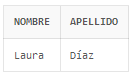
\includegraphics[width=1\linewidth]{img/Consulta_1.png}
\end{figure}

\newpage

\subsection{Listado de las reservas confirmadas en un período}
Al ejecutar el siguiente \textit{script}:
\begin{lstlisting}
SELECT r.id_reserva "Identificación de la Reserva", r.fecha_registro "Fecha de Reserva",
    c.documento "Identificación del cliente", c.nombres "Nombres", a.nombre_aerolinea "Aerolínea",
    h.nombre "Hotel", r.valor_total "Valor Reserva"
FROM reserva r
JOIN cliente c ON r.id_cliente = c.id_cliente
JOIN reserva_vuelo rv ON r.id_vuelo = rv.id_reserva_vuelo
JOIN reserva_hotel rh ON r.id_hotel = rh.id_hotel_reserva
LEFT JOIN aerolinea a ON rv.aerolinea_reservada = a.id_aerolinea
LEFT JOIN hotel h ON rh.hotel_reservado = h.id_hotel;
\end{lstlisting}

Se obtiene:

\begin{figure}[h]
    \centering
    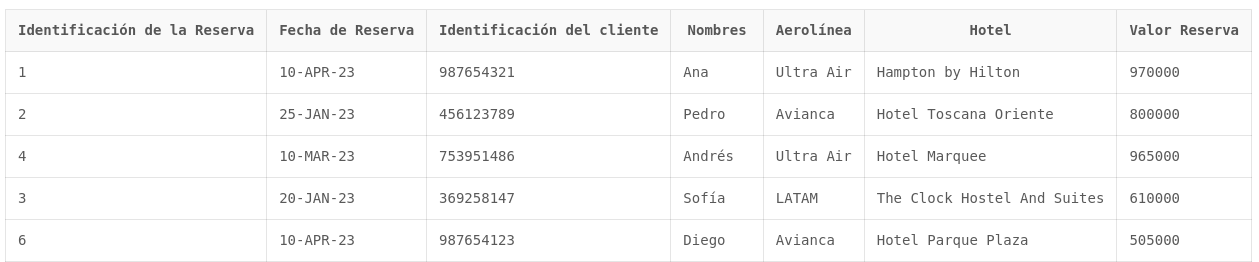
\includegraphics[width=1\linewidth]{img/Consulta_2.png}
\end{figure}

\newpage


\subsection{Top 5 de los destinos turísticos más visitados por los clientes, con base al número de reservas}
Al ejecutar el siguiente \textit{script}:
\begin{lstlisting}
SELECT c.nombre "Destinos más visitados", COUNT(r.id_reserva) "Reservas aceptadas"
FROM reserva r
JOIN ciudad c ON r.ciudad_destino = c.id_ciudad
WHERE r.fecha_registro BETWEEN TO_DATE('2020-01-01', 'YYYY-MM-DD') AND TO_DATE('2030-12-31', 'YYYY-MM-DD')
AND r.estado_reserva = 'Aceptada'
GROUP BY c.nombre
ORDER BY COUNT(r.id_reserva) DESC
FETCH FIRST 5 ROWS ONLY;
\end{lstlisting}

Se obtiene:

\begin{figure}[h]
    \centering
    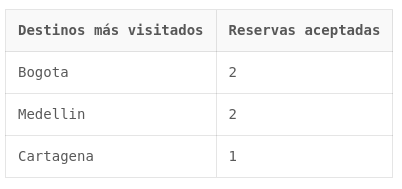
\includegraphics[width=0.75\linewidth]{img/Consulta_3.png}
\end{figure}


\newpage


\subsection{Top 5 de los destinos turísticos más visitados por los clientes, con base al número de viajeros}
Al ejecutar el siguiente \textit{script}:
\begin{lstlisting}
SELECT ciu.nombre "Destino", (COUNT(ac.id_acompañante)+1) "Número de viajeros"
FROM reserva r
JOIN cliente c ON r.id_cliente = c.id_cliente
JOIN ciudad ciu ON r.ciudad_destino = ciu.id_ciudad
LEFT JOIN acompañante ac ON c.id_cliente = ac.id_cliente
GROUP BY ciu.nombre
ORDER BY COUNT(ac.id_acompañante) DESC
FETCH FIRST 5 ROWS ONLY;
\end{lstlisting}

Se obtiene:

\begin{figure}[h]
    \centering
    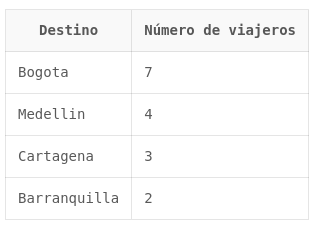
\includegraphics[width=0.75\linewidth]{img/Consulta_4.png}
\end{figure}


\newpage

\subsection{Top 5 de los destinos turísticos más visitados por los clientes, con base al volumen de ingresos por reservas}
Al ejecutar el siguiente \textit{script}:
\begin{lstlisting}
SELECT c.nombre "Destino", SUM(r.valor_total) "Ingresos por las reservas"
FROM reserva r
JOIN ciudad c ON r.ciudad_destino = c.id_ciudad
WHERE r.fecha_registro BETWEEN TO_DATE('2020-01-01', 'YYYY-MM-DD') AND TO_DATE('2030-12-31', 'YYYY-MM-DD')
GROUP BY c.nombre
ORDER BY SUM(r.valor_total) DESC
FETCH FIRST 5 ROWS ONLY;
\end{lstlisting}

Se obtiene:

\begin{figure}[h]
    \centering
    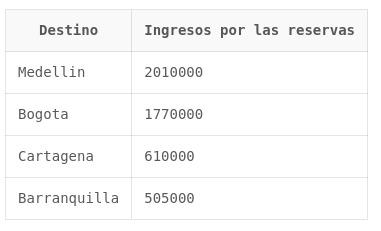
\includegraphics[width=0.75\linewidth]{img/Consulta_5.png}
\end{figure}


\newpage


\subsection{Top 5 de las aerolíneas preferidas por los clientes, con base al número de reservas}

Al ejecutar el siguiente \textit{script}:
\begin{lstlisting}
SELECT a.nombre_aerolinea "Nombre Aerolínea", COUNT(ra.id_reserva_vuelo) "Reservas confirmadas"
FROM reserva_vuelo ra
JOIN aerolinea a ON ra.aerolinea_reservada = a.id_aerolinea
WHERE ra.fecha_salida BETWEEN TO_DATE('2020-01-01', 'YYYY-MM-DD') AND TO_DATE('2030-12-31', 'YYYY-MM-DD')
AND ra.estado_solicitud_vuelo = 'Aceptado'
GROUP BY a.nombre_aerolinea
ORDER BY COUNT(ra.id_reserva_vuelo) DESC
FETCH FIRST 5 ROWS ONLY;
\end{lstlisting}

Se obtiene:

\begin{figure}[h]
    \centering
    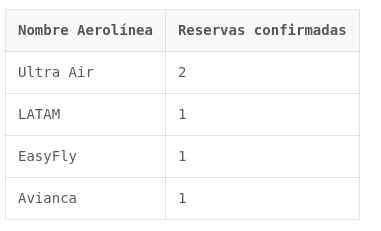
\includegraphics[width=0.75\linewidth]{img/Consulta_6.png}
\end{figure}

\newpage

\subsection{Top 5 de los hoteles preferidos por los clientes, con base al número de reservas}
Al ejecutar el siguiente \textit{script}:

\begin{lstlisting}
SELECT h.nombre "Nombre Hotel", COUNT(rh.id_hotel_reserva) "Reservas Confirmadas"
FROM reserva_hotel rh
JOIN hotel h ON rh.hotel_reservado = h.id_hotel
JOIN reserva r ON rh.id_hotel_reserva = r.id_hotel
WHERE rh.fecha_ingreso BETWEEN TO_DATE('2020-01-01', 'YYYY-MM-DD') AND TO_DATE('2030-12-31', 'YYYY-MM-DD')
AND r.estado_reserva = 'Aceptada'
GROUP BY h.nombre
ORDER BY COUNT(rh.id_hotel_reserva) DESC
FETCH FIRST 5 ROWS ONLY;
\end{lstlisting}

Se obtiene:

\begin{figure}[h]
    \centering
    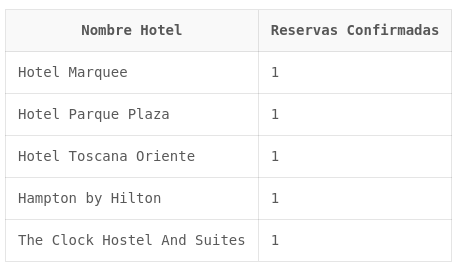
\includegraphics[width=0.75\linewidth]{img/Consulta_7.png}
\end{figure}

\newpage
\section{Construcción de paquete almacenado}
\subsection{Procedimiento para registro de cliente}
\subsection{Procedimiento para registro de solicitud de reserva de tiquetes aéreos y/o alojamiento}
\subsection{Procedimiento para registro de reservas de tiquetes aéreos y/o alojamiento}
\subsection{Procedimiento para cancelación de reserva de tiquetes aéreos y/o alojamiento}
\subsection{Función que calcule el indicador de efectividad del proceso de reservas en un período}
\subsection{Función que calcule el tiempo promedio por reserva en un período.}

\newpage
\section{Conclusiones y recomendaciones}



\newpage
\bibliographystyle{ieeetr}
\bibliography{references}


\newpage
\begin{landscape}
\section{Anexos}
\begin{figure}[H]
    \centering
    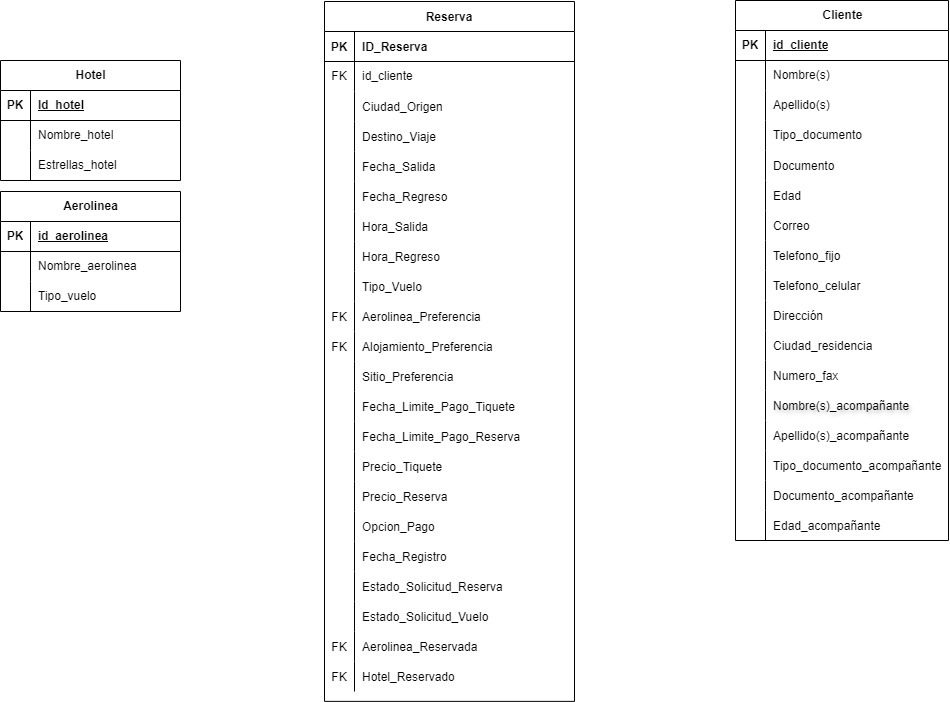
\includegraphics[scale=0.4]{img/FN1.png}
    \caption{Modelo normalizado en 1FN}
    \label{fig:NormalizacionFN1}
\end{figure}


\begin{figure}[H]
    \centering
    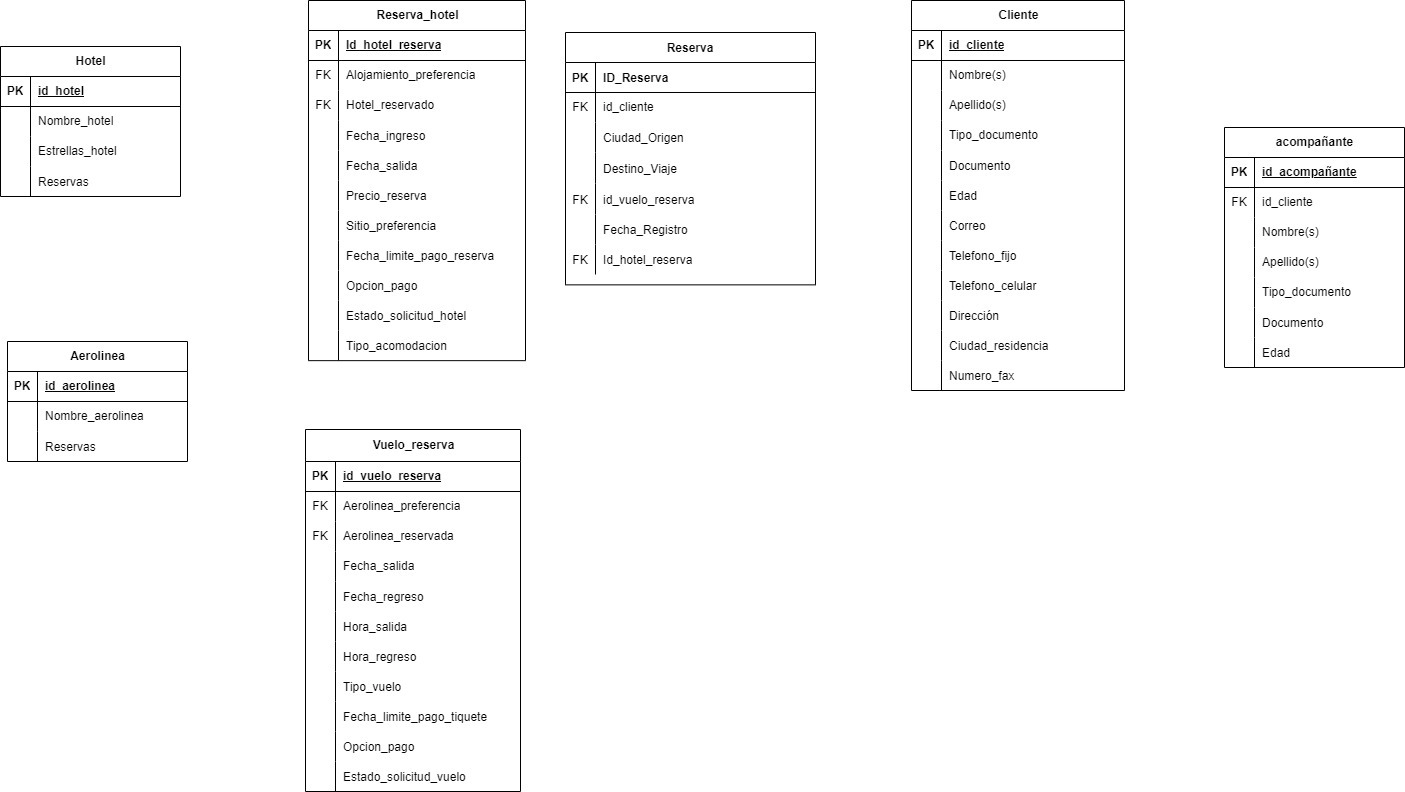
\includegraphics[width=0.9\linewidth]{img/FN2.png}
    \caption{Modelo normalizado en 2FN}
    \label{fig:Normalizacion2FN}
\end{figure}


\begin{figure}[H]
    \centering
    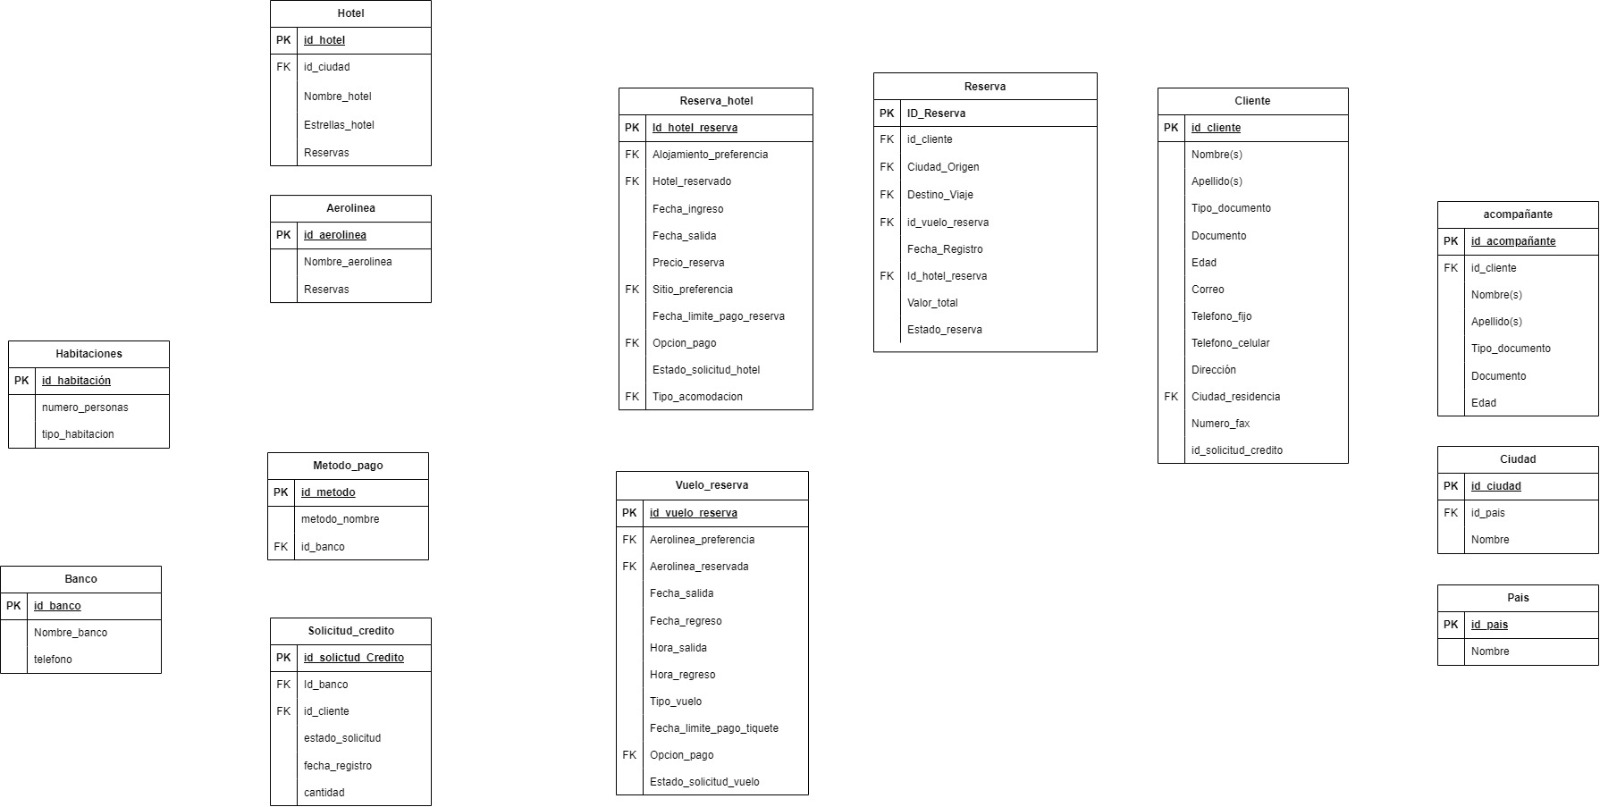
\includegraphics[width=1\linewidth]{img/FN3.png}
    \caption{Modelo normalizado en 3FN}
    \label{fig:Normalizacion3FN}
\end{figure}


\begin{figure}[H]
    \centering
    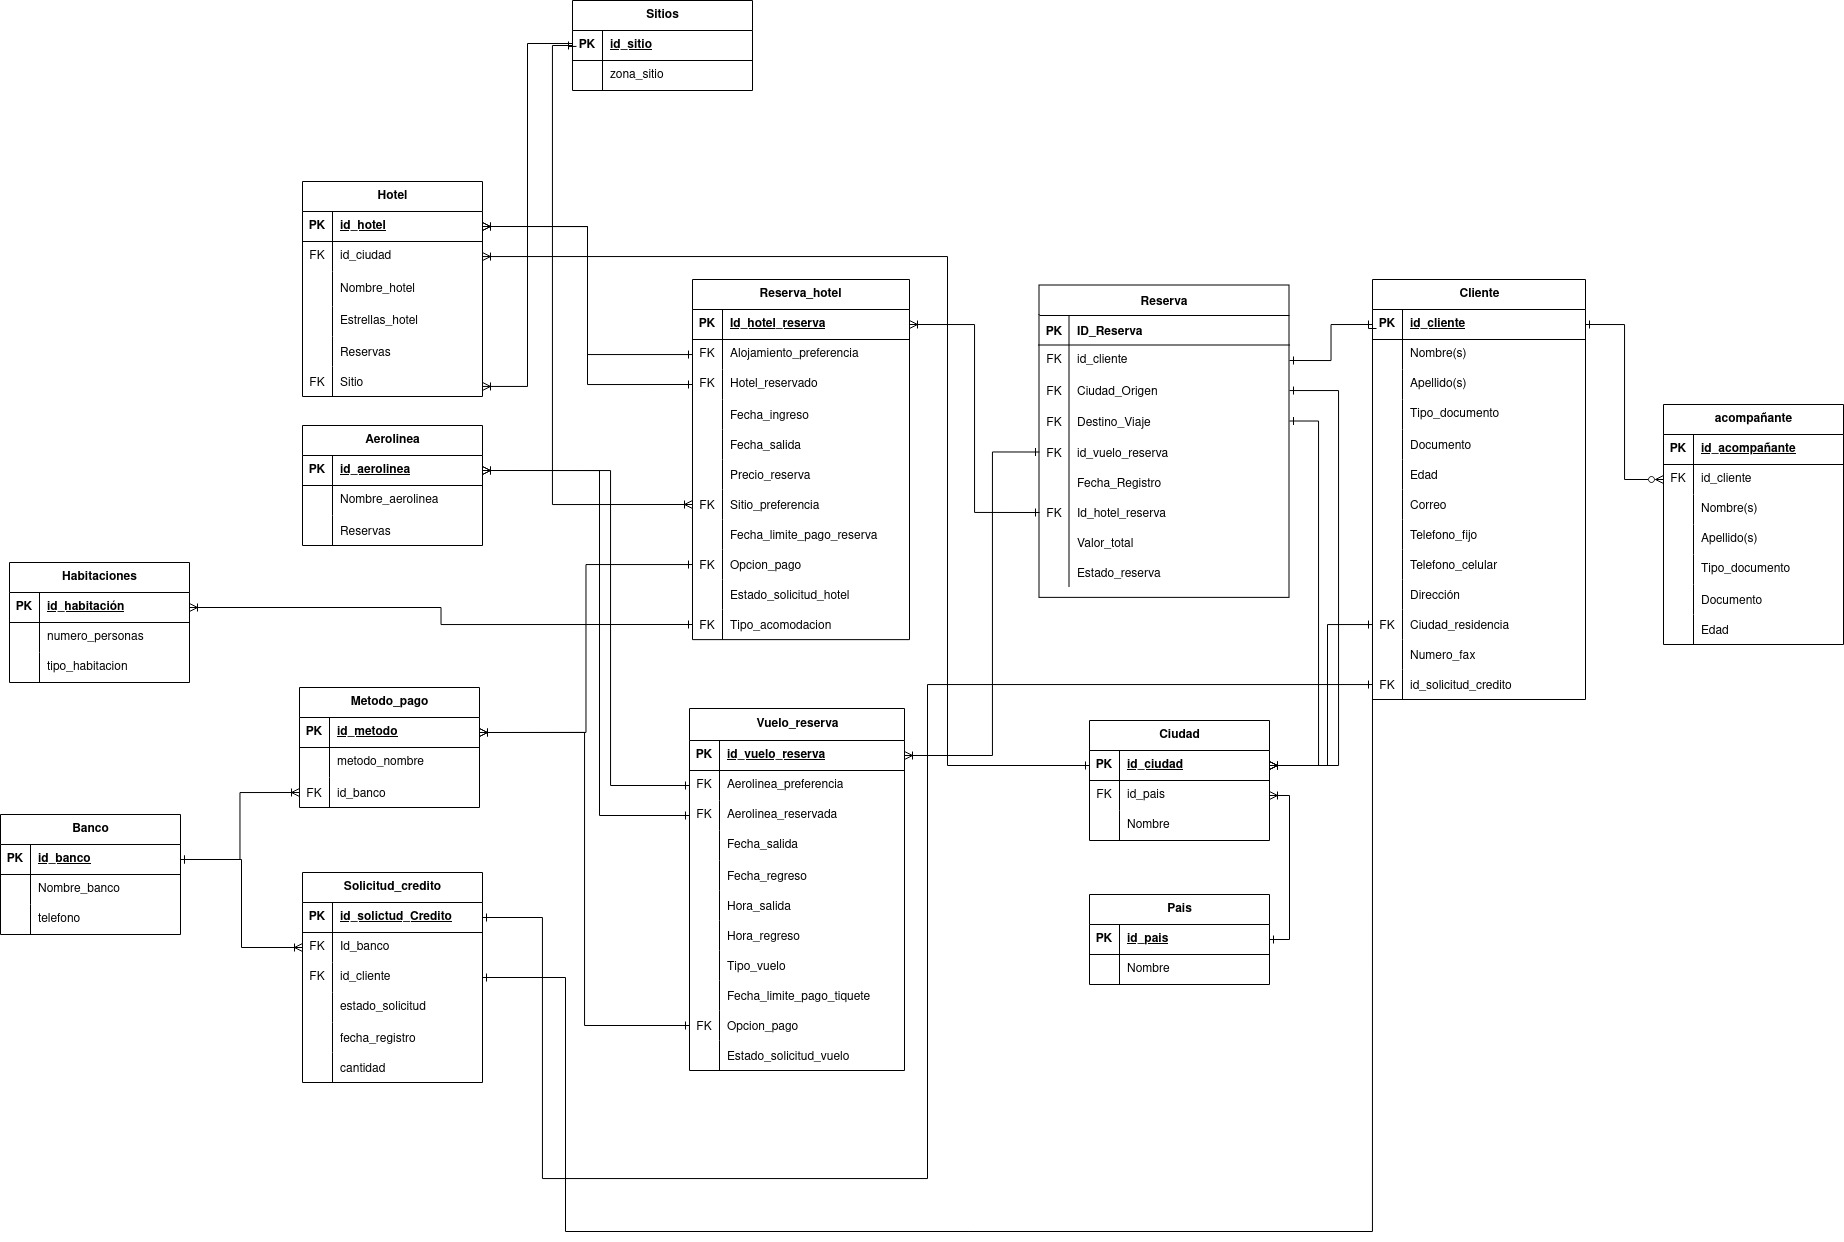
\includegraphics[width=1\linewidth]{img/ModeloEntidadRelacion.jpg}
    \caption{Modelo entidad-relación con las relaciones entre tablas.}
    \label{fig:EntidadRelacion}
\end{figure}

\newpage


\begin{longtable}{|C{0.102\linewidth}|C{0.102\linewidth}|C{0.142\linewidth}|C{0.142\linewidth}|C{0.122\linewidth}|C{0.142\linewidth}|C{0.142\linewidth}|}
\hline
\textbf{Esquema de base de datos} & \textbf{Tabla de datos a la que pertenece} & \textbf{Atributo de la tabla} & \textbf{Descripción} & \textbf{Tipo de dato} & \textbf{Rango o valores que permite el campo} & \textbf{Especificaciones y/o reglas de cálculo.} \\ \hline

TadeoTours & Sitios & zona\_sitio & Se específica el punto cardinal al cual pertenece cierto lugar geográfico & Alfanumérico & Norte, sur, oriente, occidente, nororiente, noroccidente, suroriente, suroccidente, centro. & Obligatorio. \\ \hline

TadeoTours & Hotel & Nombre\_hotel & Nombre del hotel & Alfanumérico & Todo tipo de caracteres, tienen que describir el nombre del hotel & Obligatorio. \\ \hline

TadeoTours & Hotel & Estrellas\_Hotel & Puntuación que le dan los clientes al hotel & Numérico natural & Los números naturales que se encuentren en el rango de 1 a 5 & Opcional. \\ \hline

TadeoTours & Hotel & Reservas & Cantidad de reservas que han sido registradas por el hotel & Numérico natural & Números naturales mayores o igual a 0 & Obligatorio. \\ \hline

TadeoTours & Aerolínea & Nombre\_Aerolinea & Nombre de la aerolínea & Alfanumérico & Cualquier carácter que forme del nombre de la aerolínea & Obligatorio \\ \hline

TadeoTours & Aerolínea & Reservas & Cantidad de reservas que han sido registradas por la aerolínea. & Numérico natural & Números naturales mayores o iguales a 0 & Opcional. \\ \hline

TadeoTours & Habitaciones & Número\_personas & Número de personas que permite la habitación & Numérico natural & Números naturales mayores o iguales a 1. & Obligatorio \\ \hline

TadeoTours & Habitaciones & Tipo\_habitacion & Clasificación de la habitación en tema de comodidad & Alfanumérico & Sencilla, doble o múltiple & Obligatorio. \\ \hline

TadeoTours & Metodo\_Pago & Metodo\_Nombre & Nombre del método de pago por el cual el usuario va a pagar su reserva & Alfanumérico & Efectivo, tarjeta débito, tarjeta crédito, cheque al día, cheque post-fechado, crédito. & Obligatorio. \\ \hline

TadeoTours & Banco & Nombre\_Banco & Nombre del banco & Alfanumérico & Cualquier carácter que forme parte del nombre del banco & Obligatorio \\ \hline

TadeoTours & Banco & Telefono & Teléfono de contacto del banco & Numérico natural & Generalmente, números naturales de 7 a 10 dígitos como máximo. & Obligatorio \\ \hline

TadeoTours & Solicitud\_Credito & Estado\_Solicitud & Estado en el que se encuentra la solicitud del crédito & Alfanumérico & ``Aceptado'', ``Rechazado'' o ``En espera'' & Obligatorio \\ \hline

TadeoTours & Solicitud\_Credito & Fecha\_registro & Fecha en la que se registra la solicitud del crédito en la base de daots & Fecha & Fecha en el formato YYYY\_MM\_DD & Obligatorio. \\ \hline

TadeoTours & Reserva\_Hotel & Fecha\_ingreso & Fecha a la que se espera que el cliente ingrese al hotel & Fecha & Fecha en el formato YYYY\_MM\_DD & Obligatorio. \\ \hline

TadeoTours & Reserva\_Hotel & Fecha\_salida & Fecha a la que se espera que el cliente salga del hotel & Fecha & Fecha en el formato YYYY\_MM\_DD & Obligatorio \\ \hline

TadeoTours & Reserva\_Hotel & Precio\_reserva & Precio por el que se factura la reserva del hotel & Numérico flotante & Números positivos con máximo 2 décimales de precisión & Obligatorio. \\ \hline

TadeoTours & Reserva\_Hotel & Fecha\_limite\_pago\_reserva & Fecha que el hotel asigna para el pago de la reserva & Fecha & Fecha en el formato YYYY\_MM\_DD & Opcional. \\ \hline

TadeoTours & Reserva\_Hotel & Estado\_solicitud\_hotel & Estado en el que se encuentra la solicitud de la reserva en el hotel & Alfanumérico & ``Aceptado'', ``Rechazado'' o ``En espera''. & Opcional. \\ \hline

TadeoTours & Vuelo\_reserva & Fecha\_salida & Fecha de salida del vuelo & Fecha & Fecha en el formato YYYY\_MM\_DD & Obligatorio. \\ \hline

TadeoTours & Vuelo\_reserva & Fecha\_regreso & Fecha de regreso del vuelo & Fecha & Fecha en el formato YYYY\_MM\_DD & Obligatorio. \\ \hline

TadeoTours & Vuelo\_reserva & Hora\_salida & Hora a la que va a salir el avión del aeropuerto & Tiempo & Hora de tiempo en formato 24 horas & Obligatorio \\ \hline

TadeoTours & Vuelo\_reserva & Hora\_regreso & Avión de regreso & Tiempo & Horas & Obligatorio. \\ \hline

TadeoTours & Vuelo\_reserva & Tipo\_vuelo & Categoría del vuelo & Alfanumérico & Preferencial, gerente o turista & Obligatorio. \\ \hline

TadeoTours & Vuelo\_reserva & Fecha\_limite\_pago\_tiquete & Fecha límite que asigna la aerolínea para realizar el pago del vuelo & Fecha & Fecha en el formato YYYY\_MM\_DD & Obligatorio. \\ \hline

TadeoTours & Vuelo\_reserva & Estado\_solicitud\_vuelo & Estado en el que se encuentra la solicitud del vuelo & Alfanumérico & ``Aceptado'', ``Rechazado'' o ``En espera''. & Obligatorio \\ \hline

TadeoTours & Reserva & Fecha\_registro & Fecha en la que se registra la reserva a la agencia de turismo & Fecha & Fecha en el formato YYYY\_MM\_DD & Obligatorio. \\ \hline

TadeoTours & Reserva & Valor\_total & Valor por el cual sale en total toda la reserva incluyendo reserva de hotel y de aerolínea & Numérico flotante & Números positivos con máximo 2 décimales de precisión & Obligatorio. \\ \hline

TadeoTours & Reserva & Estado\_reserva & Estado en el que se encuentra la reserva & Alfanumérico & ``Aceptado'', ``Rechazado'' o ``En espera''. & Obligatorio. \\ \hline

TadeoTours & Ciudad & Nombre & Nombre de la ciudad & Alfanumérico & Caracteres que conformen el nombre de la ciudad & Obligatorio \\ \hline

TadeoTours & País & Nombre & Nombre del país & Alfanumérico & Nombre del país & Obligatorio \\ \hline

TadeoTours & Cliente & Nombre(s) & Nombre del cliente que hace la reserva & Alfanumérico & Caracteres que conformen el nombre del cliente & Obligatorio. \\ \hline

TadeoTours & Cliente & Apellido(s) & Apellido del cliente que hace la reserva & Alfanumérico & Caracteres que conformen el apellido del cliente & Obligatorio \\ \hline

TadeoTours & Cliente & Tipo\_documento & Categoría a la que pertenece el documento de identidad del cliente & Alfanumérico & Cédula de ciudadanía (CC), Tarjeta de identidad (TI), Registro Civil (RC), Cédula de Extranjería (CE), Carné de Identidad (CI), Documento Nacional de Identidad (DNI). & Obligatorio \\ \hline

TadeoTours & Cliente & Documento & Número de identificación del cliente & Alfanumérico & Número natural & Obligatorio. \\ \hline

TadeoTours & Cliente & Edad & Edad del cliente & Numérico natural & Números naturales mayores o iguales a 18 & Obligatorio \\ \hline

TadeoTours & Cliente & Correo & Dirección de correo electrónico del usuario & Alfanumérico & Debe tener una dirección de correo electrónica asociada @dirección.com & Opcional. \\ \hline

TadeoTours & Cliente & Telefono\_fijo & Teléfono del domicilio del cliente & Numérico natural & Números naturales de 10 dígitos. & Opcional. \\ \hline

TadeoTours & Cliente & Telefono\_celular & Teléfono celular del cliente & Numérico natural & Números naturales de 10 dígitos. & Opcional. \\ \hline

TadeoTours & Cliente & Direccion & Dirección domiciliaria del cliente & Alfanumérico & Caracteres que intervienen en la dirección de vivienda del cliente & Opcional. \\ \hline

TadeoTours & Cliente & Numero\_fax & Número de dirección fax del cliente & Numérico & Números positivos & Opcional \\ \hline

TadeoTours & Acompañante & Nombre(s) & Nombre del acompañante & Alfanumérico & Caracteres que formen parte del nombre del acompañante & Obligatorio \\ \hline

TadeoTours & Acompañante & Appelido(s) & Apellido del acompañante & Alfanumérico & caracteres que formen parte del apellido del acompañante & Obligatorio \\ \hline

TadeoTours & Acompañante & Tipo\_documento & Categoría a la que pertenece el documento de identidad del acompañante & Alfanumérico & Cédula de Ciudadanía (CC), Tarjeta de Identidad (TI), Registro Civil (RC), Cédula de Extranjería (CE), Carné de Identidad (CI), Documento Nacional de Identidad (DNI). & Obligatorio. \\ \hline

TadeoTours & Acompañante & Documento & Número de identificación del acompañante & Alfanumérico & Número natural & Obligatorio. \\ \hline

TadeoTours & Acompañante & Edad & Edad del acompañante & Numérico natural & Números naturales mayores a 0 & Obligatorio \\ \hline

\caption{Diccionario de datos del esquema de la base de datos}
\label{tab:diccionario}

\end{longtable}


\end{landscape}

\end{document}
